\documentclass[12pt, a4paper, oneside]{ctexart}
\usepackage{amsmath, amsthm, amssymb, bm, color, graphicx, hyperref, mathrsfs, enumerate, setspace}
\usepackage{geometry}
\usepackage{booktabs}
\usepackage{tikz,pgfplots}
%\usepgfplotslibrary{external}
%\tikzexternalize
\pgfplotsset{width=8cm,compat=1.9}
\usepackage{float}
\usepackage{listings}
\usepackage{lastpage}
\usepackage{caption,subcaption}
\usepackage{fancyhdr}%导入fancyhdr包
\definecolor{mygreen}{RGB}{28,172,0} % color values Red, Green, Blue
\definecolor{mylilas}{RGB}{170,55,241}

\lstset{language=Matlab,%
%backgroundcolor = \color{yellow!10}, % 背景色:淡黄
basicstyle = \small\ttfamily, % 基本样式 + 小号字体
rulesepcolor= \color{gray}, % 代码块边框颜色
breaklines = true, % 代码过长则换行
morekeywords={matlab2tikz},
morekeywords=[2]{1}, keywordstyle=[2]{\color{black}},
showstringspaces=false,
showspaces=false,%
tabsize=4,%
frame=lines,%
stringstyle=\color{mylilas},
keywordstyle=\color{blue}\bfseries,%
identifierstyle=\color{black},%
commentstyle=\color{mygreen},%\itshape,%
stringstyle=\color{mylilas},
numbers=left,%
numberstyle={\tiny \color{black}},% size of the numbers
numbersep=9pt % this defines how far the numbers are from the text
}

\pagestyle{fancy}
\geometry{left=2.2cm,right=2.2cm,top=2.7cm,bottom=2.7cm}
\fancyhf{}
\fancyfoot[C]{第~\thepage~页 \quad 共~\pageref*{LastPage}~页}
\renewcommand{\headrulewidth}{0pt}
\renewcommand{\footrulewidth}{0pt}

\begin{document}


\def\bs#1{{#1}}%\boldsymbol
%\thispagestyle{empty}
%\tableofcontents
%\newpage
%\setcounter{page}{1}
\section{初始值问题的单步方法数值实验}
\subsection{实验目的}
通过实验,使得学生掌握求解初值问题的四阶、三阶以及二阶的 Runge-Kutta 方法以及 Euler 法的实现,并通过编程实现算法。
\subsection{实验内容}
求解如下微分方程的数值解
$$
\begin{cases}
    y^\prime = y - \dfrac{2x}{y}, &0<x<1 \\
    y(0) = 1
\end{cases}
$$
其中计算区间为 $[0,1]$。解析解为 $y = \sqrt{1+2x}$.

分别用 Euler 前差,改进的 Euler 公式、四阶 R-K 方法以及四阶Adams显格式和预估校正格式求解该问题。

取空间步长为 $h=1/40,1/20,1/10,1/5$。然后将每一种步长下的数值解分别于解析解相比较(计算绝对误差),给出收敛阶($RR1=LOG(ER1/ERROR1)/LOG(2.0)$)并列表显示。分析计算结果。
\subsection{实验算法理论}
对于求解一阶微分方程问题:
$$
\begin{array}{l}
    y_{i}^{\prime}=f_{i}\left(x, y_{1}, \cdots, y_{m}\right) \\
    y_{i}\left(x_{0}\right)=y_{i 0} \\
    i=1,2 \cdots, m
\end{array}
$$
由初值问题的经典单步法公式可得一阶常微分方程组初值问题各阶公式:
\begin{enumerate}
    \item Euler方法
    $$y(x_{n+1}) = y(x_{n}) + h f(x_n,y(x_n))$$
    \item 二阶 R-K 方法(改进的 Euler 公式)
    $$
    \begin{array}{l}
        y_{n+1}=y_{n}+\dfrac{h}{2}\left(k_{1}+k_{2}\right) \\
        k_{1}=f\left(x_{n}, y_{n}\right) \\
        k_{2}=f\left(x_{n+1}, y_{n}+h k_{1}\right) \\
        y_{0}=y\left(x_{0}\right)
    \end{array}
    $$
    \item 四阶 R-K 方法
    $$
    \begin{array}{l}
        y_{n+1}=y_{n}+\dfrac{h}{6}\left(k_{1}+2 k_{2}+2 k_{3}+k_{4}\right) \\
        k_{1}=f\left(x_{n}, y_{n}\right) \\
        k_{2}=f\left(x_{n}+\dfrac{1}{2} h, y_{n}+\dfrac{1}{2} h k_{1}\right) \\
        k_{3}=f\left(x_{n}+\dfrac{1}{2} h, y_{n}+\dfrac{1}{2} h k_{2}\right) \\
        k_{4}=f\left(x_{n}+h, y_{n}+h k_{3}\right)
    \end{array}
    $$
    \item 四阶Adams显格式
    $$
    y_{n+1}=y_{n}+\dfrac{h}{24}\left( 55 f_{n} - 59 f_{n-1} + 37 f_{n-2} - 9 f_{n-3} \right)
    $$
    \item 四阶Adams预估校正格式
    $$
    \begin{array}{l}
        \bar y_{n+1}=y_{n}+\dfrac{h}{24}\left( 55 f_{n} - 59 f_{n-1} + 37 f_{n-2} - 9 f_{n-3} \right) \\
        y_{n+1}=y_{n}+\dfrac{h}{24} \left( 9 f(x_{n+1},\bar y_{n+1}) + 19 f_{n} - 5 f_{n-1} + f_{n-2} \right)
    \end{array}
    $$
\end{enumerate}
\subsection{实验程序}
我们编写了以下MATLAB函数,实现使用欧拉法、梯形法、四阶 R-K 方法、四阶Adams显格式或预估校正格式求解一阶常微分方程:

\lstinputlisting[title={ode}]{ode.m}

\subsection{实验结果及分析}
使用以下MATLAB脚本对上述算法进行测试:

\lstinputlisting[title={ode test}]{ode_test.m}

各迭代方法的运行结果如图1-10和表1-10所示。由于数据过多,我们仅在Euler方法的计算结果表1-2中完整展现40个节点的数据值,而在表3-10中仅保留5个数据点。

表11列出了通过估计得到的各迭代格式的收敛阶数。

\setlength{\tabcolsep}{3pt}

% Euler方法

\begin{table}[h] %并列表格
    \centering
    \footnotesize
    \begin{minipage}[t]{0.48\textwidth}\centering
    \begin{tabular}{@{}llllll@{}}
        \toprule
        $x_i$      & $h=\frac{1}{5}$  & $h=\frac{1}{10}$ & $h=\frac{1}{20}$ & $h=\frac{1}{40}$ & 精确解    \\ \midrule
        0      & 1.0000 & 1.0000 & 1.0000 & 1.0000 & 1.0000 \\
        0.0250 &     &     &     & 1.0250 & 1.0247 \\
        0.0500 &     &     & 1.0500 & 1.0494 & 1.0488 \\
        0.0750 &     &     &     & 1.0733 & 1.0724 \\
        0.1000 &     & 1.1000 & 1.0977 & 1.0966 & 1.0954 \\
        0.1250 &     &     &     & 1.1195 & 1.1180 \\
        0.1500 &     &     & 1.1435 & 1.1419 & 1.1402 \\
        0.1750 &     &     &     & 1.1638 & 1.1619 \\
        0.2000 & 1.2000 & 1.1918 & 1.1876 & 1.1854 & 1.1832 \\
        0.2250 &     &     &     & 1.2066 & 1.2042 \\
        0.2500 &     &     & 1.2301 & 1.2275 & 1.2247 \\
        0.2750 &     &     &     & 1.2480 & 1.2450 \\
        0.3000 &     & 1.2774 & 1.2713 & 1.2681 & 1.2649 \\
        0.3250 &     &     &     & 1.2880 & 1.2845 \\
        0.3500 &     &     & 1.3113 & 1.3076 & 1.3038 \\
        0.3750 &     &     &     & 1.3269 & 1.3229 \\
        0.4000 & 1.3733 & 1.3582 & 1.3501 & 1.3459 & 1.3416 \\
        0.4250 &     &     &     & 1.3647 & 1.3601 \\
        0.4500 &     &     & 1.3880 & 1.3833 & 1.3784 \\
        0.4750 &     &     &     & 1.4016 & 1.3964 \\
        0.5000 &     & 1.4351 & 1.4250 & 1.4197 & 1.4142 \\ \bottomrule
        \end{tabular}
    \end{minipage}
    %\\[12pt]%设置两个表格之间的空白行距离
    \begin{minipage}[t]{0.48\textwidth}\centering
    \begin{tabular}{@{}llllll@{}}
        \toprule
        $x_i$      & $h=\frac{1}{5}$  & $h=\frac{1}{10}$ & $h=\frac{1}{20}$ & $h=\frac{1}{40}$ & 精确解    \\ \midrule
        0.5250 &     &     &     & 1.4376 & 1.4318 \\
        0.5500 &     &     & 1.4612 & 1.4553 & 1.4491 \\
        0.5750 &     &     &     & 1.4727 & 1.4663 \\
        0.6000 & 1.5315 & 1.5090 & 1.4966 & 1.4900 & 1.4832 \\
        0.6250 &     &     &     & 1.5071 & 1.5000 \\
        0.6500 &     &     & 1.5313 & 1.5241 & 1.5166 \\
        0.6750 &     &     &     & 1.5409 & 1.5330 \\
        0.7000 &     & 1.5803 & 1.5654 & 1.5575 & 1.5492 \\
        0.7250 &     &     &     & 1.5740 & 1.5652 \\
        0.7500 &     &     & 1.5990 & 1.5903 & 1.5811 \\
        0.7750 &     &     &     & 1.6064 & 1.5969 \\
        0.8000 & 1.6811 & 1.6498 & 1.6320 & 1.6225 & 1.6125 \\
        0.8250 &     &     &     & 1.6384 & 1.6279 \\
        0.8500 &     &     & 1.6646 & 1.6542 & 1.6432 \\
        0.8750 &     &     &     & 1.6698 & 1.6583 \\
        0.9000 &     & 1.7178 & 1.6968 & 1.6854 & 1.6733 \\
        0.9250 &     &     &     & 1.7008 & 1.6882 \\
        0.9500 &     &     & 1.7286 & 1.7162 & 1.7029 \\
        0.9750 &     &     &     & 1.7314 & 1.7176 \\
        1.0000 & 1.8269 & 1.7848 & 1.7600 & 1.7465 & 1.7321 \\ \bottomrule
        \end{tabular}
    \end{minipage}
	\caption{Euler方法计算结果} \label{fig:euler1}
\end{table}

\begin{table}[h] %并列表格
    \centering
    \footnotesize
    \begin{minipage}[t]{0.48\textwidth}\centering
    \begin{tabular}{@{}llllll@{}}
    \toprule
    $x_i$      & $h=\frac{1}{5}$  & $h=\frac{1}{10}$ & $h=\frac{1}{20}$ & $h=\frac{1}{40}$ & 精确解    \\ \midrule
    0      & 0      & 0      & 0      & 0      & 1.0000 \\
    0.0250 &     &     &     & 0.0003 & 1.0247 \\
    0.0500 &     &     & 0.0012 & 0.0006 & 1.0488 \\
    0.0750 &     &     &     & 0.0009 & 1.0724 \\
    0.1000 &     & 0.0046 & 0.0023 & 0.0012 & 1.0954 \\
    0.1250 &     &     &     & 0.0014 & 1.1180 \\
    0.1500 &     &     & 0.0033 & 0.0017 & 1.1402 \\
    0.1750 &     &     &     & 0.0019 & 1.1619 \\
    0.2000 & 0.0168 & 0.0086 & 0.0044 & 0.0022 & 1.1832 \\
    0.2250 &     &     &     & 0.0024 & 1.2042 \\
    0.2500 &     &     & 0.0054 & 0.0027 & 1.2247 \\
    0.2750 &     &     &     & 0.0030 & 1.2450 \\
    0.3000 &     & 0.0125 & 0.0064 & 0.0032 & 1.2649 \\
    0.3250 &     &     &     & 0.0035 & 1.2845 \\
    0.3500 &     &     & 0.0074 & 0.0038 & 1.3038 \\
    0.3750 &     &     &     & 0.0040 & 1.3229 \\
    0.4000 & 0.0317 & 0.0166 & 0.0085 & 0.0043 & 1.3416 \\
    0.4250 &     &     &     & 0.0046 & 1.3601 \\
    0.4500 &     &     & 0.0096 & 0.0049 & 1.3784 \\
    0.4750 &     &     &     & 0.0052 & 1.3964 \\
    0.5000 &     & 0.0209 & 0.0108 & 0.0055 & 1.4142 \\ \bottomrule
    \end{tabular}
    \end{minipage}
    %\\[12pt]%设置两个表格之间的空白行距离
    \begin{minipage}[t]{0.48\textwidth}\centering
    \begin{tabular}{@{}llllll@{}}
    \toprule
    $x_i$      & $h=\frac{1}{5}$  & $h=\frac{1}{10}$ & $h=\frac{1}{20}$ & $h=\frac{1}{40}$ & 精确解    \\ \midrule
    0.5250 &     &     &     & 0.0058 & 1.4318 \\
    0.5500 &     &     & 0.0120 & 0.0061 & 1.4491 \\
    0.5750 &     &     &     & 0.0064 & 1.4663 \\
    0.6000 & 0.0483 & 0.0257 & 0.0133 & 0.0068 & 1.4832 \\
    0.6250 &     &     &     & 0.0071 & 1.5000 \\
    0.6500 &     &     & 0.0147 & 0.0075 & 1.5166 \\
    0.6750 &     &     &     & 0.0079 & 1.5330 \\
    0.7000 &     & 0.0311 & 0.0162 & 0.0083 & 1.5492 \\
    0.7250 &     &     &     & 0.0087 & 1.5652 \\
    0.7500 &     &     & 0.0178 & 0.0091 & 1.5811 \\
    0.7750 &     &     &     & 0.0096 & 1.5969 \\
    0.8000 & 0.0686 & 0.0373 & 0.0196 & 0.0100 & 1.6125 \\
    0.8250 &     &     &     & 0.0105 & 1.6279 \\
    0.8500 &     &     & 0.0214 & 0.0110 & 1.6432 \\
    0.8750 &     &     &     & 0.0115 & 1.6583 \\
    0.9000 &     & 0.0445 & 0.0235 & 0.0121 & 1.6733 \\
    0.9250 &     &     &     & 0.0126 & 1.6882 \\
    0.9500 &     &     & 0.0256 & 0.0132 & 1.7029 \\
    0.9750 &     &     &     & 0.0138 & 1.7176 \\
    1.0000 & 0.0949 & 0.0527 & 0.0280 & 0.0145 & 1.7321 \\ \bottomrule
\end{tabular}
\end{minipage}
\caption{Euler方法绝对误差} \label{fig:euler2}
\end{table}

\begin{figure}[!h]\centering\footnotesize
\begin{minipage}[t]{0.48\textwidth}\centering
\begin{tikzpicture}[every mark/.append style={mark size=1.5pt}] %tikz图片
\begin{axis}[
    %xlabel=$x$, ylabel=$y$, xmode=linear, ymode=linear,
    tick align=inside, scaled ticks=false,
    legend style={at={(1,0)},anchor=south east}
    ]
    \addplot+[smooth] plot coordinates { 
        (0,1.0000)(0.2000,1.2000)(0.4000,1.3733)(0.6000,1.5315)(0.8000,1.6811)(1.0000,1.8269)
    };
    \addlegendentry{$h=1/5$}
    \addplot+[smooth] plot coordinates {
        (0,1.0000)(0.1000,1.1000)(0.2000,1.1918)(0.3000,1.2774)(0.4000,1.3582)(0.5000,1.4351)(0.6000,1.5090)(0.7000,1.5803)(0.8000,1.6498)(0.9000,1.7178)(1.0000,1.7848)
    };
    \addlegendentry{$h=1/10$}
    \addplot+[smooth] plot coordinates {
        (0,1.0000)(0.0500,1.0500)(0.1000,1.0977)(0.1500,1.1435)(0.2000,1.1876)(0.2500,1.2301)(0.3000,1.2713)(0.3500,1.3113)(0.4000,1.3501)(0.4500,1.3880)(0.5000,1.4250)(0.5500,1.4612)(0.6000,1.4966)(0.6500,1.5313)(0.7000,1.5654)(0.7500,1.5990)(0.8000,1.6320)(0.8500,1.6646)(0.9000,1.6968)(0.9500,1.7286)(1.0000,1.7600)
    };
    \addlegendentry{$h=1/20$}
    \addplot+[smooth] plot coordinates {
        (0,1.0000)(0.0250,1.0250)(0.0500,1.0494)(0.0750,1.0733)(0.1000,1.0966)(0.1250,1.1195)(0.1500,1.1419)(0.1750,1.1638)(0.2000,1.1854)(0.2250,1.2066)(0.2500,1.2275)(0.2750,1.2480)(0.3000,1.2681)(0.3250,1.2880)(0.3500,1.3076)(0.3750,1.3269)(0.4000,1.3459)(0.4250,1.3647)(0.4500,1.3833)(0.4750,1.4016)(0.5000,1.4197)(0.5250,1.4376)(0.5500,1.4553)(0.5750,1.4727)(0.6000,1.4900)(0.6250,1.5071)(0.6500,1.5241)(0.6750,1.5409)(0.7000,1.5575)(0.7250,1.5740)(0.7500,1.5903)(0.7750,1.6064)(0.8000,1.6225)(0.8250,1.6384)(0.8500,1.6542)(0.8750,1.6698)(0.9000,1.6854)(0.9250,1.7008)(0.9500,1.7162)(0.9750,1.7314)(1.0000,1.7465)
    };
    \addlegendentry{$h=1/40$}
    \addplot+[smooth] plot coordinates {
        (0,1.0000)(0.0250,1.0247)(0.0500,1.0488)(0.0750,1.0724)(0.1000,1.0954)(0.1250,1.1180)(0.1500,1.1402)(0.1750,1.1619)(0.2000,1.1832)(0.2250,1.2042)(0.2500,1.2247)(0.2750,1.2450)(0.3000,1.2649)(0.3250,1.2845)(0.3500,1.3038)(0.3750,1.3229)(0.4000,1.3416)(0.4250,1.3601)(0.4500,1.3784)(0.4750,1.3964)(0.5000,1.4142)(0.5250,1.4318)(0.5500,1.4491)(0.5750,1.4663)(0.6000,1.4832)(0.6250,1.5000)(0.6500,1.5166)(0.6750,1.5330)(0.7000,1.5492)(0.7250,1.5652)(0.7500,1.5811)(0.7750,1.5969)(0.8000,1.6125)(0.8250,1.6279)(0.8500,1.6432)(0.8750,1.6583)(0.9000,1.6733)(0.9250,1.6882)(0.9500,1.7029)(0.9750,1.7176)(1.0000,1.7321)
    };
    \addlegendentry{精确解}
\end{axis}
\end{tikzpicture}
\caption{Euler方法计算结果}
\end{minipage}
\begin{minipage}[t]{0.48\textwidth}\centering
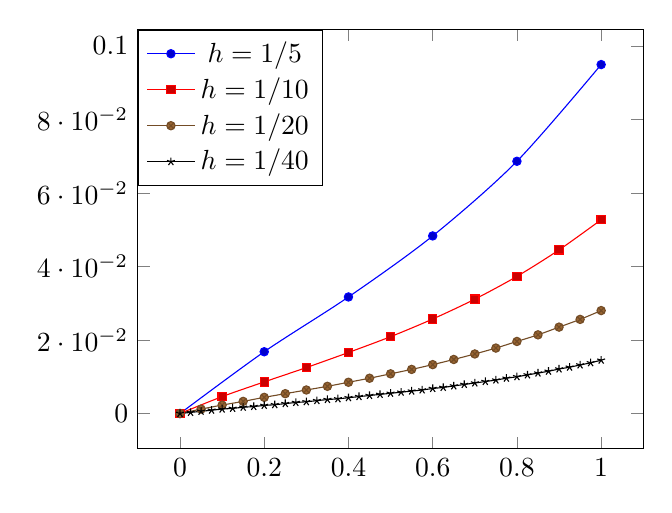
\begin{tikzpicture}[every mark/.append style={mark size=1.5pt}] %tikz图片
\begin{axis}[
    %xlabel=$x$, ylabel=$y$, xmode=linear, ymode=linear,
    tick align=inside, scaled ticks=false,
    legend style={at={(0,1)},anchor=north west}
    ]
    \addplot+[smooth] plot coordinates { 
        (0,0)(0.2000,0.0168)(0.4000,0.0317)(0.6000,0.0483)(0.8000,0.0686)(1.0000,0.0949)
    };
    \addlegendentry{$h=1/5$}
    \addplot+[smooth] plot coordinates {
        (0,0)(0.1000,0.0046)(0.2000,0.0086)(0.3000,0.0125)(0.4000,0.0166)(0.5000,0.0209)(0.6000,0.0257)(0.7000,0.0311)(0.8000,0.0373)(0.9000,0.0445)(1.0000,0.0527)
    };
    \addlegendentry{$h=1/10$}
    \addplot+[smooth] plot coordinates {
        (0,0)(0.0500,0.0012)(0.1000,0.0023)(0.1500,0.0033)(0.2000,0.0044)(0.2500,0.0054)(0.3000,0.0064)(0.3500,0.0074)(0.4000,0.0085)(0.4500,0.0096)(0.5000,0.0108)(0.5500,0.0120)(0.6000,0.0133)(0.6500,0.0147)(0.7000,0.0162)(0.7500,0.0178)(0.8000,0.0196)(0.8500,0.0214)(0.9000,0.0235)(0.9500,0.0256)(1.0000,0.0280)
    };
    \addlegendentry{$h=1/20$}
    \addplot+[smooth] plot coordinates {
        (0,0)(0.0250,0.0003)(0.0500,0.0006)(0.0750,0.0009)(0.1000,0.0012)(0.1250,0.0014)(0.1500,0.0017)(0.1750,0.0019)(0.2000,0.0022)(0.2250,0.0024)(0.2500,0.0027)(0.2750,0.0030)(0.3000,0.0032)(0.3250,0.0035)(0.3500,0.0038)(0.3750,0.0040)(0.4000,0.0043)(0.4250,0.0046)(0.4500,0.0049)(0.4750,0.0052)(0.5000,0.0055)(0.5250,0.0058)(0.5500,0.0061)(0.5750,0.0064)(0.6000,0.0068)(0.6250,0.0071)(0.6500,0.0075)(0.6750,0.0079)(0.7000,0.0083)(0.7250,0.0087)(0.7500,0.0091)(0.7750,0.0096)(0.8000,0.0100)(0.8250,0.0105)(0.8500,0.0110)(0.8750,0.0115)(0.9000,0.0121)(0.9250,0.0126)(0.9500,0.0132)(0.9750,0.0138)(1.0000,0.0145)
    };
    \addlegendentry{$h=1/40$}
\end{axis}
\end{tikzpicture}
\caption{Euler方法绝对误差}
\end{minipage}
\end{figure}

% 改进的Euler方法

\begin{table}[h] %并列表格
    \centering
    \footnotesize
    \begin{minipage}[t]{0.48\textwidth}\centering
    \begin{tabular}{@{}llllll@{}}
        \toprule
        $x_i$      & $h=\frac{1}{5}$  & $h=\frac{1}{10}$ & $h=\frac{1}{20}$ & $h=\frac{1}{40}$ & 精确解    \\ \midrule 
        0      & 1.0000 & 1.0000 & 1.0000 & 1.0000 & 1.0000 \\
        0.2000 & 1.1867 & 1.1841 & 1.1834 & 1.1833 & 1.1832 \\
        0.4000 & 1.3483 & 1.3434 & 1.3421 & 1.3417 & 1.3416 \\
        0.6000 & 1.4937 & 1.4860 & 1.4839 & 1.4834 & 1.4832 \\
        0.8000 & 1.6279 & 1.6165 & 1.6135 & 1.6127 & 1.6125 \\
        1.0000 & 1.7542 & 1.7379 & 1.7335 & 1.7324 & 1.7321 \\ \bottomrule
        \end{tabular}
	\caption{改进的Euler方法计算结果} \label{fig:euler21}
    \end{minipage}
    %\\[12pt]%设置两个表格之间的空白行距离
    \begin{minipage}[t]{0.48\textwidth}\centering
    \begin{tabular}{@{}llllll@{}}
        \toprule
        $x_i$      & $h=\frac{1}{5}$  & $h=\frac{1}{10}$ & $h=\frac{1}{20}$ & $h=\frac{1}{40}$ & 精确解    \\ \midrule 
        0      & 0      & 0      & 0      & 0      & 1.0000 \\
        0.2000 & 0.0035 & 0.0009 & 0.0002 & 0.0001 & 1.1832 \\
        0.4000 & 0.0067 & 0.0017 & 0.0004 & 0.0001 & 1.3416 \\
        0.6000 & 0.0105 & 0.0027 & 0.0007 & 0.0002 & 1.4832 \\
        0.8000 & 0.0154 & 0.0040 & 0.0010 & 0.0003 & 1.6125 \\
        1.0000 & 0.0222 & 0.0058 & 0.0015 & 0.0004 & 1.7321 \\ \bottomrule
        \end{tabular}
	\caption{改进的Euler方法绝对误差} \label{fig:euler22}
    \end{minipage}
\end{table}

\begin{figure}[!h]\centering\footnotesize
\begin{minipage}[t]{0.48\textwidth}\centering
\begin{tikzpicture}[every mark/.append style={mark size=1.5pt}] %tikz图片
    \begin{axis}[
    %xlabel=$x$, ylabel=$y$, xmode=linear, ymode=linear,
    tick align=inside, scaled ticks=false,
    legend style={at={(1,0)},anchor=south east}
    ]
    \addplot+[smooth] plot coordinates { 
        (0,1.0000)(0.2000,1.1867)(0.4000,1.3483)(0.6000,1.4937)(0.8000,1.6279)(1.0000,1.7542)
    };
    \addlegendentry{$h=1/5$}
    \addplot+[smooth] plot coordinates {
        (0,1.0000)(0.1000,1.0959)(0.2000,1.1841)(0.3000,1.2662)(0.4000,1.3434)(0.5000,1.4164)(0.6000,1.4860)(0.7000,1.5525)(0.8000,1.6165)(0.9000,1.6782)(1.0000,1.7379)
    };
    \addlegendentry{$h=1/10$}
    \addplot+[smooth] plot coordinates {
        (0,1.0000)(0.0500,1.0489)(0.1000,1.0956)(0.1500,1.1403)(0.2000,1.1834)(0.2500,1.2250)(0.3000,1.2652)(0.3500,1.3042)(0.4000,1.3421)(0.4500,1.3789)(0.5000,1.4148)(0.5500,1.4498)(0.6000,1.4839)(0.6500,1.5173)(0.7000,1.5500)(0.7500,1.5821)(0.8000,1.6135)(0.8500,1.6443)(0.9000,1.6746)(0.9500,1.7043)(1.0000,1.7335)
    };
    \addlegendentry{$h=1/20$}
    \addplot+[smooth] plot coordinates {
        (0,1.0000)(0.0250,1.0247)(0.0500,1.0488)(0.0750,1.0724)(0.1000,1.0955)(0.1250,1.1181)(0.1500,1.1402)(0.1750,1.1619)(0.2000,1.1833)(0.2250,1.2042)(0.2500,1.2248)(0.2750,1.2451)(0.3000,1.2650)(0.3250,1.2846)(0.3500,1.3039)(0.3750,1.3230)(0.4000,1.3417)(0.4250,1.3603)(0.4500,1.3785)(0.4750,1.3966)(0.5000,1.4144)(0.5250,1.4319)(0.5500,1.4493)(0.5750,1.4665)(0.6000,1.4834)(0.6250,1.5002)(0.6500,1.5168)(0.6750,1.5332)(0.7000,1.5494)(0.7250,1.5655)(0.7500,1.5814)(0.7750,1.5971)(0.8000,1.6127)(0.8250,1.6282)(0.8500,1.6434)(0.8750,1.6586)(0.9000,1.6736)(0.9250,1.6885)(0.9500,1.7033)(0.9750,1.7179)(1.0000,1.7324)
    };
    \addlegendentry{$h=1/40$}
    \addplot+[smooth] plot coordinates {
        (0,1.0000)(0.0250,1.0247)(0.0500,1.0488)(0.0750,1.0724)(0.1000,1.0954)(0.1250,1.1180)(0.1500,1.1402)(0.1750,1.1619)(0.2000,1.1832)(0.2250,1.2042)(0.2500,1.2247)(0.2750,1.2450)(0.3000,1.2649)(0.3250,1.2845)(0.3500,1.3038)(0.3750,1.3229)(0.4000,1.3416)(0.4250,1.3601)(0.4500,1.3784)(0.4750,1.3964)(0.5000,1.4142)(0.5250,1.4318)(0.5500,1.4491)(0.5750,1.4663)(0.6000,1.4832)(0.6250,1.5000)(0.6500,1.5166)(0.6750,1.5330)(0.7000,1.5492)(0.7250,1.5652)(0.7500,1.5811)(0.7750,1.5969)(0.8000,1.6125)(0.8250,1.6279)(0.8500,1.6432)(0.8750,1.6583)(0.9000,1.6733)(0.9250,1.6882)(0.9500,1.7029)(0.9750,1.7176)(1.0000,1.7321)
    };
    \addlegendentry{精确解}
\end{axis}
\end{tikzpicture}
\caption{改进的Euler方法计算结果}
\end{minipage}
\begin{minipage}[t]{0.48\textwidth}\centering
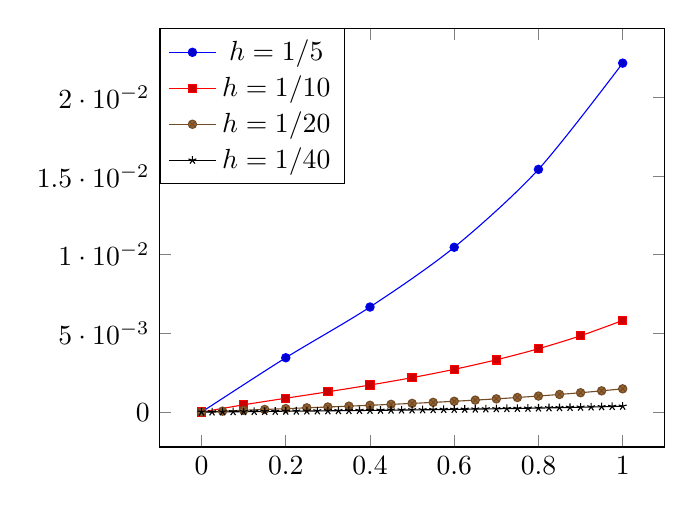
\begin{tikzpicture}[every mark/.append style={mark size=1.5pt}] %tikz图片
\begin{axis}[
    %xlabel=$x$, ylabel=$y$, xmode=linear, ymode=linear,
    tick align=inside, scaled ticks=false,
    legend style={at={(0,1)},anchor=north west}
    ]
    \addplot+[smooth] plot coordinates { 
        (0,0)(0.2000,3.4507e-03)(0.4000,6.6715e-03)(0.6000,1.0464e-02)(0.8000,1.5410e-02)(1.0000,2.2154e-02)
    };
    \addlegendentry{$h=1/5$}
    \addplot+[smooth] plot coordinates {
        (0,0)(0.1000,4.6398e-04)(0.2000,8.8061e-04)(0.3000,1.2903e-03)(0.4000,1.7194e-03)(0.5000,2.1884e-03)(0.6000,2.7159e-03)(0.7000,3.3208e-03)(0.8000,4.0232e-03)(0.9000,4.8463e-03)(1.0000,5.8166e-03)
    };
    \addlegendentry{$h=1/10$}
    \addplot+[smooth] plot coordinates {
        (0,0)(0.0500,6.0199e-05)(0.1000,1.1600e-04)(0.1500,1.6917e-04)(0.2000,2.2103e-04)(0.2500,2.7262e-04)(0.3000,3.2479e-04)(0.3500,3.7828e-04)(0.4000,4.3376e-04)(0.4500,4.9182e-04)(0.5000,5.5306e-04)(0.5500,6.1806e-04)(0.6000,6.8741e-04)(0.6500,7.6171e-04)(0.7000,8.4158e-04)(0.7500,9.2770e-04)(0.8000,1.0208e-03)(0.8500,1.1216e-03)(0.9000,1.2309e-03)(0.9500,1.3497e-03)(1.0000,1.4788e-03)
    };
    \addlegendentry{$h=1/20$}
    \addplot+[smooth] plot coordinates {
        (0,0)(0.0250,7.6673e-06)(0.0500,1.5006e-05)(0.0750,2.2082e-05)(0.1000,2.8953e-05)(0.1250,3.5669e-05)(0.1500,4.2271e-05)(0.1750,4.8796e-05)(0.2000,5.5280e-05)(0.2250,6.1750e-05)(0.2500,6.8236e-05)(0.2750,7.4761e-05)(0.3000,8.1350e-05)(0.3250,8.8024e-05)(0.3500,9.4804e-05)(0.3750,1.0171e-04)(0.4000,1.0876e-04)(0.4250,1.1598e-04)(0.4500,1.2338e-04)(0.4750,1.3098e-04)(0.5000,1.3880e-04)(0.5250,1.4685e-04)(0.5500,1.5516e-04)(0.5750,1.6375e-04)(0.6000,1.7263e-04)(0.6250,1.8182e-04)(0.6500,1.9134e-04)(0.6750,2.0122e-04)(0.7000,2.1146e-04)(0.7250,2.2211e-04)(0.7500,2.3316e-04)(0.7750,2.4466e-04)(0.8000,2.5661e-04)(0.8250,2.6906e-04)(0.8500,2.8201e-04)(0.8750,2.9550e-04)(0.9000,3.0956e-04)(0.9250,3.2422e-04)(0.9500,3.3949e-04)(0.9750,3.5543e-04)(1.0000,3.7205e-04)
    };
    \addlegendentry{$h=1/40$}
\end{axis}
\end{tikzpicture}
\caption{改进的Euler方法绝对误差}
\end{minipage}
\end{figure}

% 四阶R-K方法

\begin{table}[h] %并列表格
    \centering
    \footnotesize
    \begin{minipage}[t]{0.48\textwidth}\centering
    \begin{tabular}{@{}llllll@{}}
        \toprule
        $x_i$      & $h=\frac{1}{5}$  & $h=\frac{1}{10}$ & $h=\frac{1}{20}$ & $h=\frac{1}{40}$ & 精确解    \\ \midrule 
        0      & 1.0000 & 1.0000 & 1.0000 & 1.0000 & 1.0000 \\
        0.2000 & 1.1832 & 1.1832 & 1.1832 & 1.1832 & 1.1832 \\
        0.4000 & 1.3417 & 1.3416 & 1.3416 & 1.3416 & 1.3416 \\
        0.6000 & 1.4833 & 1.4832 & 1.4832 & 1.4832 & 1.4832 \\
        0.8000 & 1.6125 & 1.6125 & 1.6125 & 1.6125 & 1.6125 \\
        1.0000 & 1.7321 & 1.7321 & 1.7321 & 1.7321 & 1.7321 \\ \bottomrule
        \end{tabular}
	\caption{四阶R-K方法计算结果} \label{fig:rk41}
    \end{minipage}
    %\\[12pt]%设置两个表格之间的空白行距离
    \begin{minipage}[t]{0.48\textwidth}\centering
    \begin{tabular}{@{}llllll@{}}
        \toprule
        $x_i$      & $h=\frac{1}{5}$  & $h=\frac{1}{10}$ & $h=\frac{1}{20}$ & $h=\frac{1}{40}$ & 精确解    \\ \midrule 
        0      & 0      & 0      & 0      & 0      & 1.0000 \\
        0.2000 & 0.0000 & 0.0000 & 0.0000 & 0.0000 & 1.1832 \\
        0.4000 & 0.0000 & 0.0000 & 0.0000 & 0.0000 & 1.3416 \\
        0.6000 & 0.0000 & 0.0000 & 0.0000 & 0.0000 & 1.4832 \\
        0.8000 & 0.0001 & 0.0000 & 0.0000 & 0.0000 & 1.6125 \\
        1.0000 & 0.0001 & 0.0000 & 0.0000 & 0.0000 & 1.7321 \\ \bottomrule
        \end{tabular}
	\caption{四阶R-K方法绝对误差} \label{fig:rk42}
    \end{minipage}
\end{table}

\begin{figure}[!h]\centering\footnotesize
    \begin{minipage}[t]{0.48\textwidth}\centering
    \begin{tikzpicture}[every mark/.append style={mark size=1.5pt}] %tikz图片
    \begin{axis}[
        %xlabel=$x$, ylabel=$y$, xmode=linear, ymode=linear,
        tick align=inside, scaled ticks=false,
        legend style={at={(1,0)},anchor=south east}
    ]
    \addplot+[smooth] plot coordinates { 
        (0,1.0000)(0.2000,1.1832)(0.4000,1.3417)(0.6000,1.4833)(0.8000,1.6125)(1.0000,1.7321)
    };
    \addlegendentry{$h=1/5$}
    \addplot+[smooth] plot coordinates {
        (0,1.0000)(0.1000,1.0954)(0.2000,1.1832)(0.3000,1.2649)(0.4000,1.3416)(0.5000,1.4142)(0.6000,1.4832)(0.7000,1.5492)(0.8000,1.6125)(0.9000,1.6733)(1.0000,1.7321)
    };
    \addlegendentry{$h=1/10$}
    \addplot+[smooth] plot coordinates {
        (0,1.0000)(0.0500,1.0488)(0.1000,1.0954)(0.1500,1.1402)(0.2000,1.1832)(0.2500,1.2247)(0.3000,1.2649)(0.3500,1.3038)(0.4000,1.3416)(0.4500,1.3784)(0.5000,1.4142)(0.5500,1.4491)(0.6000,1.4832)(0.6500,1.5166)(0.7000,1.5492)(0.7500,1.5811)(0.8000,1.6125)(0.8500,1.6432)(0.9000,1.6733)(0.9500,1.7029)(1.0000,1.7321)
    };
    \addlegendentry{$h=1/20$}
    \addplot+[smooth] plot coordinates {
        (0,1.0000)(0.0250,1.0247)(0.0500,1.0488)(0.0750,1.0724)(0.1000,1.0954)(0.1250,1.1180)(0.1500,1.1402)(0.1750,1.1619)(0.2000,1.1832)(0.2250,1.2042)(0.2500,1.2247)(0.2750,1.2450)(0.3000,1.2649)(0.3250,1.2845)(0.3500,1.3038)(0.3750,1.3229)(0.4000,1.3416)(0.4250,1.3601)(0.4500,1.3784)(0.4750,1.3964)(0.5000,1.4142)(0.5250,1.4318)(0.5500,1.4491)(0.5750,1.4663)(0.6000,1.4832)(0.6250,1.5000)(0.6500,1.5166)(0.6750,1.5330)(0.7000,1.5492)(0.7250,1.5652)(0.7500,1.5811)(0.7750,1.5969)(0.8000,1.6125)(0.8250,1.6279)(0.8500,1.6432)(0.8750,1.6583)(0.9000,1.6733)(0.9250,1.6882)(0.9500,1.7029)(0.9750,1.7176)(1.0000,1.7321)
    };
    \addlegendentry{$h=1/40$}
    \addplot+[smooth] plot coordinates {
        (0,1.0000)(0.0250,1.0247)(0.0500,1.0488)(0.0750,1.0724)(0.1000,1.0954)(0.1250,1.1180)(0.1500,1.1402)(0.1750,1.1619)(0.2000,1.1832)(0.2250,1.2042)(0.2500,1.2247)(0.2750,1.2450)(0.3000,1.2649)(0.3250,1.2845)(0.3500,1.3038)(0.3750,1.3229)(0.4000,1.3416)(0.4250,1.3601)(0.4500,1.3784)(0.4750,1.3964)(0.5000,1.4142)(0.5250,1.4318)(0.5500,1.4491)(0.5750,1.4663)(0.6000,1.4832)(0.6250,1.5000)(0.6500,1.5166)(0.6750,1.5330)(0.7000,1.5492)(0.7250,1.5652)(0.7500,1.5811)(0.7750,1.5969)(0.8000,1.6125)(0.8250,1.6279)(0.8500,1.6432)(0.8750,1.6583)(0.9000,1.6733)(0.9250,1.6882)(0.9500,1.7029)(0.9750,1.7176)(1.0000,1.7321)
    };
    \addlegendentry{精确解}
    \end{axis}
    \end{tikzpicture}
    \caption{四阶R-K方法计算结果}
    \end{minipage}
    \begin{minipage}[t]{0.48\textwidth}\centering
    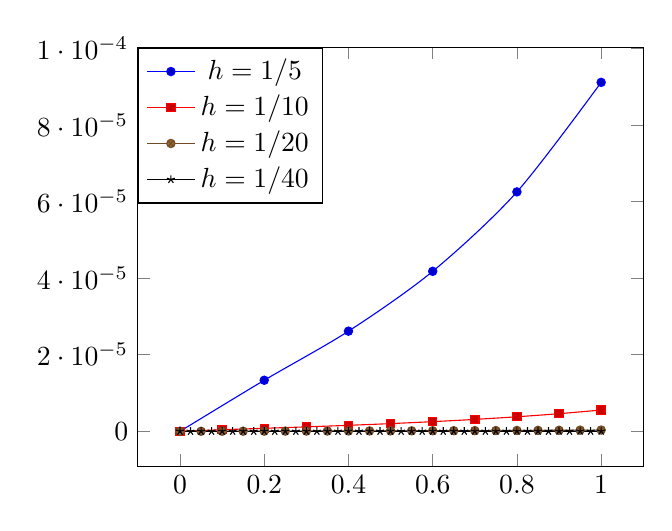
\begin{tikzpicture}[every mark/.append style={mark size=1.5pt}] %tikz图片
    \begin{axis}[
        %xlabel=$x$, ylabel=$y$, xmode=linear, ymode=linear,
        tick align=inside, scaled ticks=false,
        legend style={at={(0,1)},anchor=north west}
    ]
    \addplot+[smooth] plot coordinates { 
        (0,0)(0.2000,1.3331e-05)(0.4000,2.6143e-05)(0.6000,4.1761e-05)(0.8000,6.2492e-05)(1.0000,9.1075e-05)
    };
    \addlegendentry{$h=1/5$}
    \addplot+[smooth] plot coordinates {
        (0,0)(0.1000,4.1668e-07)(0.2000,7.8889e-07)(0.3000,1.1643e-06)(0.4000,1.5673e-06)(0.5000,2.0155e-06)(0.6000,2.5254e-06)(0.7000,3.1138e-06)(0.8000,3.8000e-06)(0.9000,4.6059e-06)(1.0000,5.5576e-06)
    };
    \addlegendentry{$h=1/10$}
    \addplot+[smooth] plot coordinates {
        (0,0)(0.0500,1.3021e-08)(0.1000,2.4874e-08)(0.1500,3.6198e-08)(0.2000,4.7379e-08)(0.2500,5.8675e-08)(0.3000,7.0275e-08)(0.3500,8.2332e-08)(0.4000,9.4977e-08)(0.4500,1.0833e-07)(0.5000,1.2252e-07)(0.5500,1.3767e-07)(0.6000,1.5389e-07)(0.6500,1.7133e-07)(0.7000,1.9012e-07)(0.7500,2.1041e-07)(0.8000,2.3237e-07)(0.8500,2.5616e-07)(0.9000,2.8199e-07)(0.9500,3.1005e-07)(1.0000,3.4057e-07)
    };
    \addlegendentry{$h=1/20$}
    \addplot+[smooth] plot coordinates {
        (0,0)(0.0250,4.0690e-10)(0.0500,7.9029e-10)(0.0750,1.1572e-09)(0.1000,1.5130e-09)(0.1250,1.8616e-09)(0.1500,2.2062e-09)(0.1750,2.5493e-09)(0.2000,2.8929e-09)(0.2250,3.2388e-09)(0.2500,3.5883e-09)(0.2750,3.9429e-09)(0.3000,4.3037e-09)(0.3250,4.6718e-09)(0.3500,5.0483e-09)(0.3750,5.4339e-09)(0.4000,5.8299e-09)(0.4250,6.2369e-09)(0.4500,6.6561e-09)(0.4750,7.0882e-09)(0.5000,7.5342e-09)(0.5250,7.9950e-09)(0.5500,8.4716e-09)(0.5750,8.9650e-09)(0.6000,9.4762e-09)(0.6250,1.0006e-08)(0.6500,1.0556e-08)(0.6750,1.1127e-08)(0.7000,1.1719e-08)(0.7250,1.2335e-08)(0.7500,1.2976e-08)(0.7750,1.3642e-08)(0.8000,1.4336e-08)(0.8250,1.5057e-08)(0.8500,1.5809e-08)(0.8750,1.6592e-08)(0.9000,1.7408e-08)(0.9250,1.8259e-08)(0.9500,1.9146e-08)(0.9750,2.0071e-08)(1.0000,2.1036e-08)
    };
    \addlegendentry{$h=1/40$}
    \end{axis}
    \end{tikzpicture}
    \caption{四阶R-K方法绝对误差}
    \end{minipage}
\end{figure}

% 四阶Adams显格式

\begin{table}[h] %并列表格
    \centering
    \footnotesize
    \begin{minipage}[t]{0.48\textwidth}\centering
    \begin{tabular}{@{}llllll@{}}
        \toprule
        $x_i$      & $h=\frac{1}{5}$  & $h=\frac{1}{10}$ & $h=\frac{1}{20}$ & $h=\frac{1}{40}$ & 精确解    \\ \midrule 
        0      & 1.0000 & 1.0000 & 1.0000 & 1.0000 & 1.0000 \\
        0.2000 & 1.1832 & 1.1832 & 1.1832 & 1.1832 & 1.1832 \\
        0.4000 & 1.3417 & 1.3416 & 1.3416 & 1.3416 & 1.3416 \\
        0.6000 & 1.4833 & 1.4830 & 1.4832 & 1.4832 & 1.4832 \\
        0.8000 & 1.6114 & 1.6121 & 1.6124 & 1.6124 & 1.6125 \\
        1.0000 & 1.7298 & 1.7316 & 1.7320 & 1.7320 & 1.7321 \\ \bottomrule
        \end{tabular}
	\caption{四阶Adams显格式计算结果} \label{fig:adams11}
    \end{minipage}
    %\\[12pt]%设置两个表格之间的空白行距离
    \begin{minipage}[t]{0.48\textwidth}\centering
    \begin{tabular}{@{}llllll@{}}
        \toprule
        $x_i$      & $h=\frac{1}{5}$  & $h=\frac{1}{10}$ & $h=\frac{1}{20}$ & $h=\frac{1}{40}$ & 精确解    \\ \midrule 
        0      & 0       & 0       & 0       & 0       & 1.0000 \\
        0.2000 & 0.0000  & 0.0000  & -0.0000 & -0.0000 & 1.1832 \\
        0.4000 & 0.0000  & -0.0001 & -0.0000 & -0.0000 & 1.3416 \\
        0.6000 & 0.0000  & -0.0002 & -0.0000 & -0.0000 & 1.4832 \\
        0.8000 & -0.0010 & -0.0003 & -0.0000 & -0.0000 & 1.6125 \\
        1.0000 & -0.0022 & -0.0005 & -0.0001 & -0.0000 & 1.7321 \\ \bottomrule
        \end{tabular}
	\caption{四阶Adams显格式绝对误差} \label{fig:adams12}
    \end{minipage}
\end{table}

\begin{figure}[!h]\centering\footnotesize
    \begin{minipage}[t]{0.48\textwidth}\centering
    \begin{tikzpicture}[every mark/.append style={mark size=1.5pt}] %tikz图片
    \begin{axis}[
        %xlabel=$x$, ylabel=$y$, xmode=linear, ymode=linear,
        tick align=inside, scaled ticks=false,
        legend style={at={(1,0)},anchor=south east}
    ]
    \addplot+[smooth] plot coordinates { 
        (0,1.0000)(0.2000,1.1832)(0.4000,1.3417)(0.6000,1.4833)(0.8000,1.6114)(1.0000,1.7298)
    };
    \addlegendentry{$h=1/5$}
    \addplot+[smooth] plot coordinates {
        (0,1.0000)(0.1000,1.0954)(0.2000,1.1832)(0.3000,1.2649)(0.4000,1.3416)(0.5000,1.4140)(0.6000,1.4830)(0.7000,1.5489)(0.8000,1.6121)(0.9000,1.6729)(1.0000,1.7316)
    };
    \addlegendentry{$h=1/10$}
    \addplot+[smooth] plot coordinates {
        (0,1.0000)(0.0500,1.0488)(0.1000,1.0954)(0.1500,1.1402)(0.2000,1.1832)(0.2500,1.2247)(0.3000,1.2649)(0.3500,1.3038)(0.4000,1.3416)(0.4500,1.3784)(0.5000,1.4142)(0.5500,1.4491)(0.6000,1.4832)(0.6500,1.5165)(0.7000,1.5492)(0.7500,1.5811)(0.8000,1.6124)(0.8500,1.6431)(0.9000,1.6733)(0.9500,1.7029)(1.0000,1.7320)
    };
    \addlegendentry{$h=1/20$}
    \addplot+[smooth] plot coordinates {
        (0,1.0000)(0.0250,1.0247)(0.0500,1.0488)(0.0750,1.0724)(0.1000,1.0954)(0.1250,1.1180)(0.1500,1.1402)(0.1750,1.1619)(0.2000,1.1832)(0.2250,1.2042)(0.2500,1.2247)(0.2750,1.2450)(0.3000,1.2649)(0.3250,1.2845)(0.3500,1.3038)(0.3750,1.3229)(0.4000,1.3416)(0.4250,1.3601)(0.4500,1.3784)(0.4750,1.3964)(0.5000,1.4142)(0.5250,1.4318)(0.5500,1.4491)(0.5750,1.4663)(0.6000,1.4832)(0.6250,1.5000)(0.6500,1.5166)(0.6750,1.5330)(0.7000,1.5492)(0.7250,1.5652)(0.7500,1.5811)(0.7750,1.5969)(0.8000,1.6124)(0.8250,1.6279)(0.8500,1.6432)(0.8750,1.6583)(0.9000,1.6733)(0.9250,1.6882)(0.9500,1.7029)(0.9750,1.7176)(1.0000,1.7320)
    };
    \addlegendentry{$h=1/40$}
    \addplot+[smooth] plot coordinates {
        (0,1.0000)(0.0250,1.0247)(0.0500,1.0488)(0.0750,1.0724)(0.1000,1.0954)(0.1250,1.1180)(0.1500,1.1402)(0.1750,1.1619)(0.2000,1.1832)(0.2250,1.2042)(0.2500,1.2247)(0.2750,1.2450)(0.3000,1.2649)(0.3250,1.2845)(0.3500,1.3038)(0.3750,1.3229)(0.4000,1.3416)(0.4250,1.3601)(0.4500,1.3784)(0.4750,1.3964)(0.5000,1.4142)(0.5250,1.4318)(0.5500,1.4491)(0.5750,1.4663)(0.6000,1.4832)(0.6250,1.5000)(0.6500,1.5166)(0.6750,1.5330)(0.7000,1.5492)(0.7250,1.5652)(0.7500,1.5811)(0.7750,1.5969)(0.8000,1.6125)(0.8250,1.6279)(0.8500,1.6432)(0.8750,1.6583)(0.9000,1.6733)(0.9250,1.6882)(0.9500,1.7029)(0.9750,1.7176)(1.0000,1.7321)
    };
    \addlegendentry{精确解}
    \end{axis}
    \end{tikzpicture}
    \caption{四阶Adams显格式计算结果}
    \end{minipage}
    \begin{minipage}[t]{0.48\textwidth}\centering
    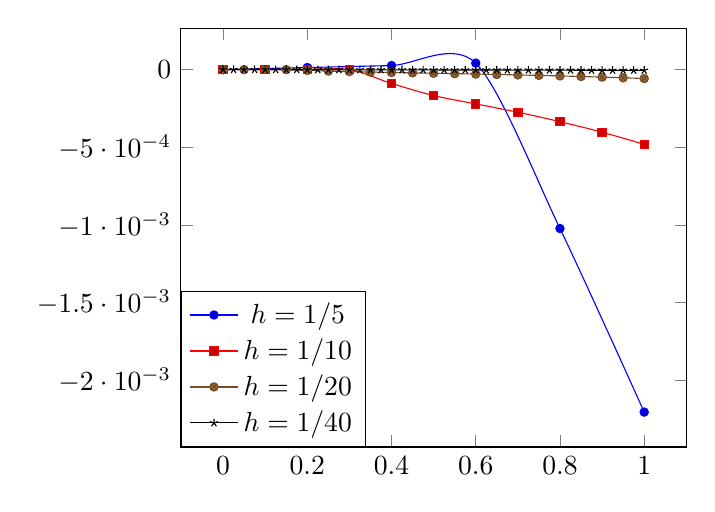
\begin{tikzpicture}[every mark/.append style={mark size=1.5pt}] %tikz图片
    \begin{axis}[
        %xlabel=$x$, ylabel=$y$, xmode=linear, ymode=linear,
        tick align=inside, scaled ticks=false,
        legend style={at={(0,0)},anchor=south west}
    ]
    \addplot+[smooth] plot coordinates { 
        (0,0)(0.2000,1.3331e-05)(0.4000,2.6143e-05)(0.6000,4.1761e-05)(0.8000,-1.0230e-03)(1.0000,-2.2050e-03)
    };
    \addlegendentry{$h=1/5$}
    \addplot+[smooth] plot coordinates {
        (0,0)(0.1000,4.1668e-07)(0.2000,7.8889e-07)(0.3000,1.1643e-06)(0.4000,-8.9027e-05)(0.5000,-1.6714e-04)(0.6000,-2.2079e-04)(0.7000,-2.7446e-04)(0.8000,-3.3512e-04)(0.9000,-4.0302e-04)(1.0000,-4.8105e-04)
    };
    \addlegendentry{$h=1/10$}
    \addplot+[smooth] plot coordinates {
        (0,0)(0.0500,1.3021e-08)(0.1000,2.4874e-08)(0.1500,3.6198e-08)(0.2000,-5.2384e-06)(0.2500,-9.6744e-06)(0.3000,-1.2933e-05)(0.3500,-1.5812e-05)(0.4000,-1.8473e-05)(0.4500,-2.0996e-05)(0.5000,-2.3481e-05)(0.5500,-2.6004e-05)(0.6000,-2.8616e-05)(0.6500,-3.1362e-05)(0.7000,-3.4281e-05)(0.7500,-3.7406e-05)(0.8000,-4.0774e-05)(0.8500,-4.4416e-05)(0.9000,-4.8367e-05)(0.9500,-5.2663e-05)(1.0000,-5.7341e-05)
    };
    \addlegendentry{$h=1/20$}
    \addplot+[smooth] plot coordinates {
        (0,0)(0.0250,4.0690e-10)(0.0500,7.9029e-10)(0.0750,1.1572e-09)(0.1000,-2.3602e-07)(0.1250,-4.4583e-07)(0.1500,-6.1953e-07)(0.1750,-7.7399e-07)(0.2000,-9.1243e-07)(0.2250,-1.0381e-06)(0.2500,-1.1540e-06)(0.2750,-1.2627e-06)(0.3000,-1.3659e-06)(0.3250,-1.4652e-06)(0.3500,-1.5620e-06)(0.3750,-1.6571e-06)(0.4000,-1.7514e-06)(0.4250,-1.8458e-06)(0.4500,-1.9409e-06)(0.4750,-2.0371e-06)(0.5000,-2.1351e-06)(0.5250,-2.2353e-06)(0.5500,-2.3380e-06)(0.5750,-2.4436e-06)(0.6000,-2.5526e-06)(0.6250,-2.6652e-06)(0.6500,-2.7818e-06)(0.6750,-2.9027e-06)(0.7000,-3.0282e-06)(0.7250,-3.1587e-06)(0.7500,-3.2944e-06)(0.7750,-3.4357e-06)(0.8000,-3.5829e-06)(0.8250,-3.7363e-06)(0.8500,-3.8964e-06)(0.8750,-4.0633e-06)(0.9000,-4.2375e-06)(0.9250,-4.4194e-06)(0.9500,-4.6093e-06)(0.9750,-4.8077e-06)(1.0000,-5.0150e-06)
    };
    \addlegendentry{$h=1/40$}
    \end{axis}
\end{tikzpicture}
\caption{四阶Adams显格式绝对误差}
\end{minipage}
\end{figure}
    
% 四阶Adams预估校正格式

\begin{table}[h] %并列表格
    \centering
    \footnotesize
    \begin{minipage}[t]{0.48\textwidth}\centering
    \begin{tabular}{@{}llllll@{}}
        \toprule
        $x_i$      & $h=\frac{1}{5}$  & $h=\frac{1}{10}$ & $h=\frac{1}{20}$ & $h=\frac{1}{40}$ & 精确解    \\ \midrule 
        0      & 1.0000 & 1.0000 & 1.0000 & 1.0000 & 1.0000 \\
        0.2000 & 1.1832 & 1.1832 & 1.1832 & 1.1832 & 1.1832 \\
        0.4000 & 1.3417 & 1.3416 & 1.3416 & 1.3416 & 1.3416 \\
        0.6000 & 1.4833 & 1.4832 & 1.4832 & 1.4832 & 1.4832 \\
        0.8000 & 1.6124 & 1.6125 & 1.6125 & 1.6125 & 1.6125 \\
        1.0000 & 1.7320 & 1.7321 & 1.7321 & 1.7321 & 1.7321 \\ \bottomrule
        \end{tabular}
	\caption{四阶Adams预估校正格式计算结果} \label{fig:adams21}
    \end{minipage}
    %\\[12pt]%设置两个表格之间的空白行距离
    \begin{minipage}[t]{0.48\textwidth}\centering
    \begin{tabular}{@{}llllll@{}}
        \toprule
        $x_i$      & $h=\frac{1}{5}$  & $h=\frac{1}{10}$ & $h=\frac{1}{20}$ & $h=\frac{1}{40}$ & 精确解    \\ \midrule 
        0      & 0       & 0       & 0      & 0      & 1.0000 \\
        0.2000 & 0.0000  & 0.0000  & 0.0000 & 0.0000 & 1.1832 \\
        0.4000 & 0.0000  & 0.0000  & 0.0000 & 0.0000 & 1.3416 \\
        0.6000 & 0.0000  & 0.0000  & 0.0000 & 0.0000 & 1.4832 \\
        0.8000 & -0.0000 & -0.0000 & 0.0000 & 0.0000 & 1.6125 \\
        1.0000 & -0.0001 & -0.0000 & 0.0000 & 0.0000 & 1.7321 \\ \bottomrule
        \end{tabular}
	\caption{四阶Adams预估校正格式绝对误差} \label{fig:adams22}
    \end{minipage}
\end{table}

\begin{figure}[!h]\centering\footnotesize
    \begin{minipage}[t]{0.48\textwidth}\centering
    \begin{tikzpicture}[every mark/.append style={mark size=1.5pt}] %tikz图片
    \begin{axis}[
        %xlabel=$x$, ylabel=$y$, xmode=linear, ymode=linear,
        tick align=inside, scaled ticks=false,
        legend style={at={(1,0)},anchor=south east}
    ]
    \addplot+[smooth] plot coordinates { 
        (0,1.0000)(0.2000,1.1832)(0.4000,1.3417)(0.6000,1.4833)(0.8000,1.6124)(1.0000,1.7320)
    };
    \addlegendentry{$h=1/5$}
    \addplot+[smooth] plot coordinates {
        (0,1.0000)(0.1000,1.0954)(0.2000,1.1832)(0.3000,1.2649)(0.4000,1.3416)(0.5000,1.4142)(0.6000,1.4832)(0.7000,1.5492)(0.8000,1.6125)(0.9000,1.6733)(1.0000,1.7321)
    };
    \addlegendentry{$h=1/10$}
    \addplot+[smooth] plot coordinates {
        (0,1.0000)(0.0500,1.0488)(0.1000,1.0954)(0.1500,1.1402)(0.2000,1.1832)(0.2500,1.2247)(0.3000,1.2649)(0.3500,1.3038)(0.4000,1.3416)(0.4500,1.3784)(0.5000,1.4142)(0.5500,1.4491)(0.6000,1.4832)(0.6500,1.5166)(0.7000,1.5492)(0.7500,1.5811)(0.8000,1.6125)(0.8500,1.6432)(0.9000,1.6733)(0.9500,1.7029)(1.0000,1.7321)
    };
    \addlegendentry{$h=1/20$}
    \addplot+[smooth] plot coordinates {
        (0,1.0000)(0.0250,1.0247)(0.0500,1.0488)(0.0750,1.0724)(0.1000,1.0954)(0.1250,1.1180)(0.1500,1.1402)(0.1750,1.1619)(0.2000,1.1832)(0.2250,1.2042)(0.2500,1.2247)(0.2750,1.2450)(0.3000,1.2649)(0.3250,1.2845)(0.3500,1.3038)(0.3750,1.3229)(0.4000,1.3416)(0.4250,1.3601)(0.4500,1.3784)(0.4750,1.3964)(0.5000,1.4142)(0.5250,1.4318)(0.5500,1.4491)(0.5750,1.4663)(0.6000,1.4832)(0.6250,1.5000)(0.6500,1.5166)(0.6750,1.5330)(0.7000,1.5492)(0.7250,1.5652)(0.7500,1.5811)(0.7750,1.5969)(0.8000,1.6125)(0.8250,1.6279)(0.8500,1.6432)(0.8750,1.6583)(0.9000,1.6733)(0.9250,1.6882)(0.9500,1.7029)(0.9750,1.7176)(1.0000,1.7321)
    };
    \addlegendentry{$h=1/40$}
    \addplot+[smooth] plot coordinates {
        (0,1.0000)(0.0250,1.0247)(0.0500,1.0488)(0.0750,1.0724)(0.1000,1.0954)(0.1250,1.1180)(0.1500,1.1402)(0.1750,1.1619)(0.2000,1.1832)(0.2250,1.2042)(0.2500,1.2247)(0.2750,1.2450)(0.3000,1.2649)(0.3250,1.2845)(0.3500,1.3038)(0.3750,1.3229)(0.4000,1.3416)(0.4250,1.3601)(0.4500,1.3784)(0.4750,1.3964)(0.5000,1.4142)(0.5250,1.4318)(0.5500,1.4491)(0.5750,1.4663)(0.6000,1.4832)(0.6250,1.5000)(0.6500,1.5166)(0.6750,1.5330)(0.7000,1.5492)(0.7250,1.5652)(0.7500,1.5811)(0.7750,1.5969)(0.8000,1.6125)(0.8250,1.6279)(0.8500,1.6432)(0.8750,1.6583)(0.9000,1.6733)(0.9250,1.6882)(0.9500,1.7029)(0.9750,1.7176)(1.0000,1.7321)
    };
    \addlegendentry{精确解}
    \end{axis}
    \end{tikzpicture}
    \caption{四阶Adams预估校正格式计算结果}
    \end{minipage}
    \begin{minipage}[t]{0.48\textwidth}\centering
    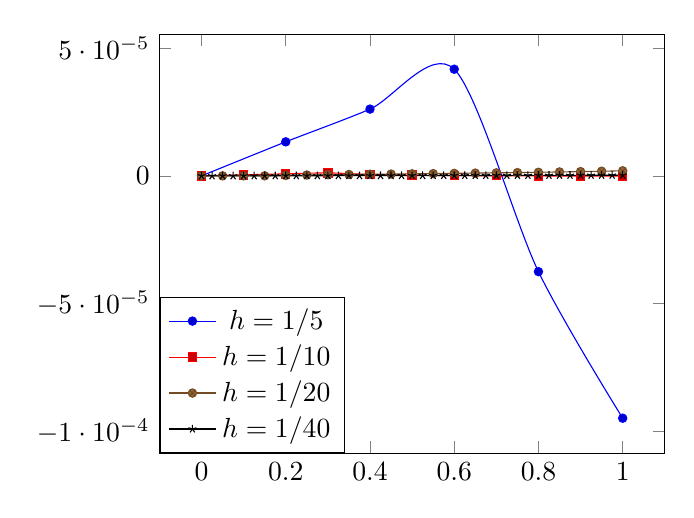
\begin{tikzpicture}[every mark/.append style={mark size=1.5pt}] %tikz图片
    \begin{axis}[
        %xlabel=$x$, ylabel=$y$, xmode=linear, ymode=linear,
        tick align=inside, scaled ticks=false,
        legend style={at={(0,0)},anchor=south west}
    ]
    \addplot+[smooth] plot coordinates { 
        (0,0)(0.2000,1.3331e-05)(0.4000,2.6143e-05)(0.6000,4.1761e-05)(0.8000,-3.7483e-05)(1.0000,-9.4844e-05)
    };
    \addlegendentry{$h=1/5$}
    \addplot+[smooth] plot coordinates {
        (0,0)(0.1000,4.1668e-07)(0.2000,7.8889e-07)(0.3000,1.1643e-06)(0.4000,5.7069e-07)(0.5000,2.7109e-07)(0.6000,1.2683e-07)(0.7000,4.2004e-08)(0.8000,-1.3185e-08)(0.9000,-5.3713e-08)(1.0000,-8.7694e-08)
    };
    \addlegendentry{$h=1/10$}
    \addplot+[smooth] plot coordinates {
        (0,0)(0.0500,1.3021e-08)(0.1000,2.4874e-08)(0.1500,3.6198e-08)(0.2000,2.1031e-07)(0.2500,3.4714e-07)(0.3000,4.5920e-07)(0.3500,5.5711e-07)(0.4000,6.4705e-07)(0.4500,7.3327e-07)(0.5000,8.1879e-07)(0.5500,9.0586e-07)(0.6000,9.9625e-07)(0.6500,1.0914e-06)(0.7000,1.1927e-06)(0.7500,1.3013e-06)(0.8000,1.4183e-06)(0.8500,1.5449e-06)(0.9000,1.6822e-06)(0.9500,1.8316e-06)(1.0000,1.9943e-06)
    };
    \addlegendentry{$h=1/20$}
    \addplot+[smooth] plot coordinates {
        (0,0)(0.0250,4.0690e-10)(0.0500,7.9029e-10)(0.0750,1.1572e-09)(0.1000,1.3945e-08)(0.1250,2.4882e-08)(0.1500,3.4329e-08)(0.1750,4.2647e-08)(0.2000,5.0095e-08)(0.2250,5.6875e-08)(0.2500,6.3145e-08)(0.2750,6.9028e-08)(0.3000,7.4625e-08)(0.3250,8.0018e-08)(0.3500,8.5273e-08)(0.3750,9.0445e-08)(0.4000,9.5580e-08)(0.4250,1.0072e-07)(0.4500,1.0590e-07)(0.4750,1.1114e-07)(0.5000,1.1648e-07)(0.5250,1.2194e-07)(0.5500,1.2754e-07)(0.5750,1.3330e-07)(0.6000,1.3925e-07)(0.6250,1.4539e-07)(0.6500,1.5175e-07)(0.6750,1.5835e-07)(0.7000,1.6519e-07)(0.7250,1.7231e-07)(0.7500,1.7972e-07)(0.7750,1.8742e-07)(0.8000,1.9545e-07)(0.8250,2.0383e-07)(0.8500,2.1256e-07)(0.8750,2.2166e-07)(0.9000,2.3117e-07)(0.9250,2.4109e-07)(0.9500,2.5145e-07)(0.9750,2.6228e-07)(1.0000,2.7358e-07)
    };
    \addlegendentry{$h=1/40$}
    \end{axis}
    \end{tikzpicture}
    \caption{四阶Adams预估校正格式绝对误差}
    \end{minipage}
\end{figure}

\begin{table}[h] %并列表格
    \centering
    \begin{tabular}{@{}cccccc@{}}
        \toprule
        算法 & Euler法 & 改进的Euler法 & 四阶R-K法 & 四阶Adams显格式 & 四阶Adams预估校正格式 \\ \midrule 
        收敛阶 & 0.9050 & 1.9653 & 4.0267 & 2.9268 & 2.8125 \\ \bottomrule
        \end{tabular}
	\caption{各迭代格式的收敛阶}
\end{table}

\end{document}





\section{抛物方程差分格式数值实验}
\subsection{实验目的}
通过实验,使得学生掌握求解抛物型方程边值问题的数值格式,并通过编程实现算法。
\subsection{实验内容}
求解如下微分方程的数值解
$$
\left\{\begin{array}{l}
    \dfrac{\partial u}{\partial t}-\dfrac{\partial^{2} u}{\partial x^{2}}=x^{2}\left(x^{2}-12\right) \mathrm e^{t}, \quad 0<x<1, \quad 0<t \leq 1 \\
    u(x, 0)=x^{4}, \quad 0 \leq x \leq 1, \\
    u(0, t)=0, \quad u(1, t)=\mathrm e^{t}, \quad 0<t \leq 1 .
\end{array}\right.
$$
解析解为$u(x, t)=x^{4} \mathrm e^t$,分别取$h_1=\dfrac{1}{5},\tau_1=\dfrac{1}{10}; h_2=\dfrac{1}{10},\tau_2=\dfrac{1}{20}; h_3=\dfrac{1}{20},\tau_3=\dfrac{1}{40}$. 列表输出节点 $(0.4,0.2i),i=1,2,\cdots,5$ 处的数值结果,精确结果以及误差。

使用 c-n 格式实现该程序。
\subsection{实验算法理论}
$$
\begin{array}{l}
    -\frac{r}{2} u_{i-1}^{k+1}+(1+r) u_{i}^{k+1}-\frac{r}{2} u_{i+1}^{k+1}=\frac{r}{2} u_{i-1}^{k}+(1-r) u_{i}^{k}+\frac{r}{2} u_{i+1}^{k}+\tau f\left(x_{i}, t_{k+\frac{1}{2}}\right)\\
    1 \leq i \leq m-1,0 \leq k \leq n-1
\end{array}
$$
详细结果参考ppt
\subsection{实验程序}

\subsection{实验结果及分析}
列表与真解比较,同时画出图形。

\begin{table}[h]
\centering\begin{tabular}{llll}
    \toprule
    节点 $(0.4,0.2i)$ & C-N 格式方法解 & 精确解 & 绝对误差 \\ \midrule
                 &          &     &      \\
                 &          &     &      \\
                 &          &     &      \\
                 &          &     &      \\
                 &          &     &      \\ \bottomrule
\end{tabular}
\end{table}

\section{双曲方程差分格式数值实验}
\subsection{实验目的}
通过实验,使得学生掌握求解双曲型方程边值问题的数值格式,并通过编程实现算法。
\subsection{实验内容}
求解如下偏微分方程的数值解
$$
\begin{cases}
    u_t+u_x = 0, &x\in[0,2] \\
    u(x,0) = \begin{cases}
        1, & 0.5\leq x\leq 1.5 \\
        0, & 0\leq x\leq 0.5, 0.5\leq x\leq 2
    \end{cases}
\end{cases}
$$
左右两端采用周期性边界条件,将[0,2]等分成20个网格,通过MATLAB程序,我们使用迎风格式,蛙跳格式、Lax-Friedrichs格式、Lax-Wendroff格式和BW格式,分别取,算至$T=2$时的各数值模拟。
精度测试(Lax-Friedrichs格式),
u(x,0)=sin(pi*x),时间取为T=2.0
计算最大模:ERROR=MAX(ERROR,ABS(UEXACT(KK)-U(KK)))
误差阶      R=LOG(ER1/ER2)/LOG(2.0d0)
注释:ER1为粗网格下的数值误差(如:n=10)
      ER2为细网格下的数值误差(如:n=20)
程序框架N=10
DO K=1,8	
 TIMET=0.d0
    INITIAL(赋初始值)
    DO I=1,NTMAX (时间层)
       赋周期边界条件
       DO J=1,N(空间层)
       ENDDO
ERROR=MAX(ERROR,ABS(UEXACT(KK)-U(KK)))(算最大误差)
       IF(K>2)
R=LOG(ER1/ER2)/LOG(2.0d0)
ENDIF
          ER1=ERROR
     ENDDO
        N=2*N
ENDDO
\subsection{实验算法理论}

\subsection{实验程序}

\subsection{实验结果及分析}

\section{Poisson方程五点格式数值实验}
\subsection{实验目的}
通过实验,使得学生掌握求解椭圆型方程边值问题的五点数值格式,并通过编程实现算法。
\subsection{实验内容}
求解如下微分方程的数值解
$$
\left\{\begin{array}{l}
    -\left(\frac{\partial^{2} u}{\partial^{2} x}+\frac{\partial^{2} u}{\partial^{2} y}\right)=\left(\pi^{2}-1\right) \mathrm e^{x} \sin (\pi y), \quad 0<x<2, \quad 0<y<1, \\
    u(0, y)=\sin (\pi y), \quad u(2, y)=\mathrm e^{2} \sin (\pi y), \quad 0 \leq y \leq 1, \\
    u(x, 0)=u(x, 1)=0, \quad 0<x<2.
\end{array}\right.
$$
解析解为$u(x,y) = \mathrm e^x \sin(\pi y)$.
使用五点格式实现该程序,网格剖分取20等份。
\subsection{实验算法理论}
$$
-\frac{u_{i-1, j}}{(\Delta x)^{2}}-\frac{u_{i+1, j}}{(\Delta x)^{2}}+2\left(\frac{1}{(\Delta x)^{2}}+\frac{1}{(\Delta y)^{2}}\right) u_{i, j}-\frac{u_{i, j-1}}{(\Delta y)^{2}}-\frac{u_{i, j+1}}{(\Delta y)^{2}}=f\left(x_{i}, y_{j}\right),
$$
右端项改为$(\pi^2-1)\mathrm e^x \sin(\pi y)$,
$$
\begin{array}{l}
    -\frac{1}{(\Delta y)^{2}}\left(\begin{array}{ccccc}
    1 & & & & \\
    & 1 & & 0 & \\
    & & \ddots & & \\
    & 0 & & 1 & \\
    & & & & 1
    \end{array}\right)\left(\begin{array}{c}
    u_{1, j-1} \\
    u_{2, j-1} \\
    \vdots \\
    u_{m-2, j-1} \\
    u_{m-1, j-1}
    \end{array}\right)-\frac{1}{(\Delta y)^{2}}\left(\begin{array}{ccccc}
    1 & & & & \\
    & 1 & & 0 & \\
    & & \ddots & & \\
    & 0 & & 1 & \\
    & & & & 1
    \end{array}\right)\left(\begin{array}{c}
    u_{1, j+1} \\
    u_{2, j+1} \\
    \vdots \\
    u_{m-2, j+1} \\
    u_{m-1, j+1}
    \end{array}\right)+\\
    \left(\begin{array}{ccccc}
    2\left(\frac{1}{(\Delta x)^{2}}+\frac{1}{(\Delta y)^{2}}\right) & -\frac{1}{(\Delta x)^{2}} & & & \\
    -\frac{1}{(\Delta x)^{2}} & 2\left(\frac{1}{(\Delta x)^{2}}+\frac{1}{(\Delta y)^{2}}\right) & -\frac{1}{(\Delta x)^{2}} & & \\
    & \ddots & \ddots & \ddots & \\
    & & -\frac{1}{(\Delta x)^{2}} & 2\left(\frac{1}{(\Delta x)^{2}}+\frac{1}{(\Delta y)^{2}}\right) & -\frac{1}{(\Delta x)^{2}} \\
    & & & -\frac{1}{(\Delta x)^{2}} & 2\left(\frac{1}{(\Delta x)^{2}}+\frac{1}{(\Delta y)^{2}}\right)
    \end{array}\right)\left(\begin{array}{c}
    u_{1, j} \\
    u_{2, j} \\
    \vdots \\
    u_{m-2, j} \\
    u_{m-1, j}
    \end{array}\right)
\end{array}
$$

记$\vec u_j = \left(\begin{array}{c}
    u_{1, j} \\
    u_{2, j} \\
    \vdots \\
    u_{m-1, j}
    \end{array}\right), 2\left(\frac{1}{(\Delta x)^{2}}+\frac{1}{(\Delta y)^{2}}\right) = \alpha, \frac{1}{(\Delta x)^{2}} = \beta, \frac{1}{(\Delta y)^{2}} = \gamma$
得到
$$
\left(\begin{array}{cccc}
    -\gamma & & & \\
    & -\gamma & & \\
    & & \ddots & \\
    & & & -\gamma
    \end{array}\right)\left(\begin{array}{c}
    u_{1, j-1} \\
    u_{2, j-1} \\
    \vdots \\
    u_{m-1, j-1}
    \end{array}\right)+\left(\begin{array}{cccc}
    \alpha & -\beta & & \\
    -\beta & \alpha & -\beta & \\
    & & \ddots & \\
    & & -\beta & \alpha
    \end{array}\right)\left(\begin{array}{c}
    u_{1, j} \\
    u_{2, j} \\
    \vdots \\
    u_{m-1, j}
    \end{array}\right)
$$    
得到
从而得到最终的关系式


\subsection{实验程序}
说明:参考文件中的m文件和pdf文件,网格采用等距剖分,套用所给程序,注意初始值以及右端项的改变。就是程序中初始值与b的形式与所给代码不同。
\subsection{实验结果及分析}
列表与真解比较,同时画出图形。